% Figure 1: method pipeline. Build: tectonic pipeline.tex
\documentclass[tikz,border=2pt,10pt]{standalone}
\usepackage[T1]{fontenc}
\usepackage{amsmath}
\usepackage{newtxtext}
\usepackage{newtxmath}
\usetikzlibrary{arrows.meta,positioning,fit,backgrounds,calc}

\newcommand{\PAL}{\mathcal{L}_{\mathrm{PAL}}}
\newcommand{\CE}{\mathcal{L}_{\mathrm{CE}}}

\definecolor{trainfill}{HTML}{DDE8F4}
\definecolor{trainline}{HTML}{3F6C9C}
\definecolor{frozenfill}{HTML}{E8E8E8}
\definecolor{frozenline}{HTML}{8C8C8C}
\definecolor{lossfill}{HTML}{FBE7D3}
\definecolor{lossline}{HTML}{B0601E}
\definecolor{dataline}{HTML}{9A9A9A}
\definecolor{arrowcol}{HTML}{4A4A4A}

\newcommand{\ftag}[1]{\\[-1pt]{\scriptsize\itshape\color{black!55}#1}}

\begin{document}
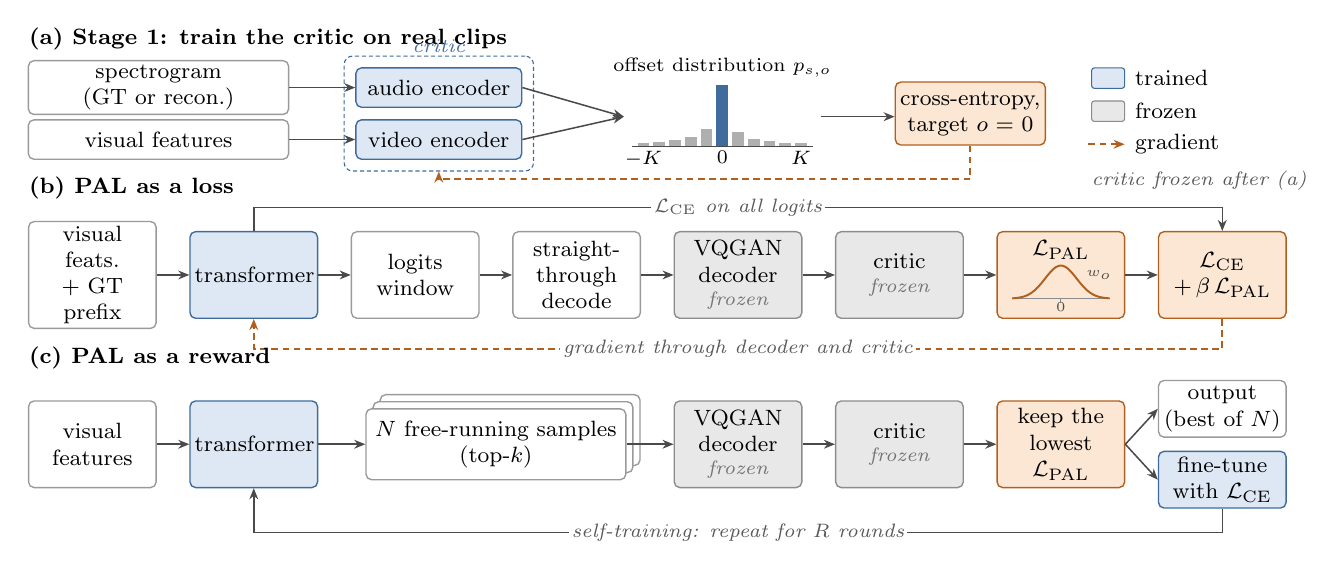
\begin{tikzpicture}[
  font=\footnotesize,
  >={Stealth[length=4pt,width=3.2pt]},
  box/.style={draw, rounded corners=2pt, line width=0.5pt, align=center,
              minimum width=1.62cm, minimum height=1.1cm, text width=1.5cm,
              inner sep=1.5pt},
  data/.style={box, draw=dataline, fill=white},
  trained/.style={box, draw=trainline, fill=trainfill},
  frozen/.style={box, draw=frozenline, fill=frozenfill},
  loss/.style={box, draw=lossline, fill=lossfill},
  flow/.style={->, draw=arrowcol, line width=0.55pt},
  grad/.style={->, draw=lossline, line width=0.6pt, dash pattern=on 2.4pt off 1.6pt},
  head/.style={anchor=west, font=\footnotesize\bfseries, inner sep=0pt},
  lane/.style={font=\scriptsize\itshape, text=black!65, fill=white, inner sep=1pt},
]

% column centres for rows (b) and (c)
\def\xa{0.85}\def\xb{2.90}\def\xc{4.95}\def\xd{7.00}
\def\xe{9.05}\def\xf{11.10}\def\xg{13.15}\def\xh{15.20}
\def\ya{0}\def\yb{-2.05}\def\yc{-4.2}

% ---------------- (a) Stage 1 ----------------
\node[head] at (0.04,\ya+0.95) {(a) Stage 1: train the critic on real clips};

\node[data, minimum width=3.3cm, text width=3.2cm, minimum height=0.5cm]
  (spec) at (1.69,\ya+0.33) {spectrogram (GT or recon.)};
\node[data, minimum width=3.3cm, text width=3.2cm, minimum height=0.5cm]
  (vis) at (1.69,\ya-0.33) {visual features};

\node[trained, minimum width=2.1cm, text width=2.0cm, minimum height=0.5cm]
  (aenc) at (5.25,\ya+0.33) {audio encoder};
\node[trained, minimum width=2.1cm, text width=2.0cm, minimum height=0.5cm]
  (venc) at (5.25,\ya-0.33) {video encoder};
\begin{scope}[on background layer]
  \node[draw=trainline, dash pattern=on 1.5pt off 1pt, rounded corners=3pt,
        inner sep=4pt, fit=(aenc)(venc)] (critic) {};
\end{scope}
\node[font=\scriptsize\itshape, text=trainline, anchor=south, inner sep=1pt]
  at (critic.north) {critic};

\draw[flow] (spec.east) -- (aenc.west);
\draw[flow] (vis.east) -- (venc.west);

% offset distribution over -K..K
\begin{scope}[shift={(8.85,\ya-0.42)}]
  \def\bw{0.15}
  \foreach \o/\h in {-5/0.05,-4/0.06,-3/0.08,-2/0.12,-1/0.22,1/0.18,2/0.10,3/0.07,4/0.05,5/0.04}{
    \fill[frozenline!70] ({\o*0.2-\bw/2},0) rectangle ({\o*0.2+\bw/2},\h);
  }
  \fill[trainline] ({-\bw/2},0) rectangle ({\bw/2},0.78);
  \draw[arrowcol, line width=0.4pt] (-1.15,0) -- (1.15,0);
  \node[font=\scriptsize, below, inner sep=1.5pt] at (-1.0,0) {$-K$};
  \node[font=\scriptsize, below, inner sep=1.5pt] at (0,0) {$0$};
  \node[font=\scriptsize, below, inner sep=1.5pt] at (1.0,0) {$K$};
  \coordinate (distW) at (-1.25,0.38);
  \coordinate (distE) at (1.25,0.38);
  \node[font=\scriptsize, align=center, anchor=south, inner sep=1pt] at (0,0.84)
    {offset distribution $p_{s,o}$};
\end{scope}
\draw[flow] (aenc.east) -- (distW);
\draw[flow] (venc.east) -- (distW);

\node[loss, minimum width=1.9cm, text width=1.8cm, minimum height=0.8cm] (ce1) at (12.0,\ya)
  {cross-entropy,\\target $o = 0$};
\draw[flow] (distE) -- (ce1.west |- distE);
\draw[grad] (ce1.south) -- ++(0,-0.42) -| (critic.south);

% legend
\begin{scope}[shift={(13.75,\ya+0.45)}]
  \node[draw=trainline, fill=trainfill, rounded corners=1pt, minimum width=0.42cm,
        minimum height=0.26cm, inner sep=0pt] at (0,0) {};
  \node[anchor=west, inner sep=1pt] at (0.3,0) {trained};
  \node[draw=frozenline, fill=frozenfill, rounded corners=1pt, minimum width=0.42cm,
        minimum height=0.26cm, inner sep=0pt] at (0,-0.42) {};
  \node[anchor=west, inner sep=1pt] at (0.3,-0.42) {frozen};
  \draw[grad] (-0.25,-0.84) -- (0.21,-0.84);
  \node[anchor=west, inner sep=1pt] at (0.3,-0.84) {gradient};
  \node[anchor=west, inner sep=1pt, text=black!65, font=\scriptsize\itshape]
    at (-0.25,-1.3) {critic frozen after (a)};
\end{scope}

% ---------------- (b) PAL as a loss ----------------
\node[head] at (0.04,\yb+1.1) {(b) PAL as a loss};

\node[data]    (b1) at (\xa,\yb) {visual feats.\\+ GT prefix};
\node[trained] (b2) at (\xb,\yb) {transformer};
\node[data]    (b3) at (\xc,\yb) {logits\\window};
\node[data]    (b4) at (\xd,\yb) {straight-\\through\\decode};
\node[frozen]  (b5) at (\xe,\yb) {VQGAN\\decoder\ftag{frozen}};
\node[frozen]  (b6) at (\xf,\yb) {critic\ftag{frozen}};
\node[loss]    (b7) at (\xg,\yb) {};
\node[anchor=north, inner sep=1pt] at ($(b7.north)+(0,-0.08)$) {$\PAL$};
\begin{scope}[shift={($(b7.center)+(0,-0.3)$)}]
  \draw[frozenline, line width=0.35pt] (-0.62,0) -- (0.62,0);
  \draw[frozenline, line width=0.35pt] (0,0) -- (0,-0.05);
  \draw[lossline, line width=0.7pt, smooth, samples=41, domain=-0.62:0.62]
    plot (\x, {0.42*exp(-(\x/0.2)^2/2)});
  \node[font=\tiny, anchor=west, inner sep=0.5pt, text=black!70] at (0.3,0.3) {$w_o$};
  \node[font=\tiny, anchor=north, inner sep=0.5pt, text=black!70] at (0,-0.03) {$0$};
\end{scope}
\node[loss]    (b8) at (\xh,\yb) {$\CE$\\$+\,\beta\,\PAL$};

\draw[flow] (b1) -- (b2);
\draw[flow] (b2) -- (b3);
\draw[flow] (b3) -- (b4);
\draw[flow] (b4) -- (b5);
\draw[flow] (b5) -- (b6);
\draw[flow] (b6) -- (b7);
\draw[flow] (b7) -- (b8);
\draw[flow] (b2.north) -- ++(0,0.3) -| node[lane, pos=0.25] {$\CE$ on all logits} (b8.north);
\draw[grad] (b8.south) -- ++(0,-0.38) -| node[lane, pos=0.25] {gradient through decoder and critic} (b2.south);

% ---------------- (c) PAL as a reward ----------------
\node[head] at (0.04,\yc+1.1) {(c) PAL as a reward};

\node[data]    (c1) at (\xa,\yc) {visual\\features};
\node[trained] (c2) at (\xb,\yc) {transformer};
% stack of N samples spanning columns c and d
\def\sx{5.975}
\foreach \k in {2,1}{
  \node[data, minimum width=3.3cm, minimum height=0.9cm, text width=3.1cm]
    at (\sx+0.09*\k,\yc+0.09*\k) {};
}
\node[data, minimum width=3.3cm, minimum height=0.9cm, text width=3.1cm]
  (c3) at (\sx,\yc) {$N$ free-running samples\\(top-$k$)};
\node[frozen]  (c5) at (\xe,\yc) {VQGAN\\decoder\ftag{frozen}};
\node[frozen]  (c6) at (\xf,\yc) {critic\ftag{frozen}};
\node[loss]    (c7) at (\xg,\yc) {keep the\\lowest $\PAL$};
\node[data, minimum height=0.72cm] (c8a) at (\xh,\yc+0.45) {output\\(best of $N$)};
\node[trained, minimum height=0.72cm] (c8b) at (\xh,\yc-0.45) {fine-tune\\with $\CE$};

\draw[flow] (c1) -- (c2);
\draw[flow] (c2) -- (c3.west);
\draw[flow] (c3) -- (c5);
\draw[flow] (c5) -- (c6);
\draw[flow] (c6) -- (c7);
\draw[flow] (c7.east) -- (c8a.west);
\draw[flow] (c7.east) -- (c8b.west);
\draw[flow] (c8b.south) -- ++(0,-0.3) -| node[lane, pos=0.25] {self-training: repeat for $R$ rounds} (c2.south);

\end{tikzpicture}
\end{document}
